\documentclass[conference]{IEEEtran}
\IEEEoverridecommandlockouts
% The preceding line is only needed to identify funding in the first footnote. If that is unneeded, please comment it out.
\usepackage{cite}
\usepackage{amsmath,amssymb,amsfonts}
\usepackage{algorithmic}
\usepackage{graphicx}
\usepackage{textcomp}
\usepackage{xcolor}
\usepackage{hyperref}
\usepackage[utf8]{inputenc}
\usepackage{float}
\usepackage [section]{placeins}


\def\BibTeX{{\rm B\kern-.05em{\sc i\kern-.025em b}\kern-.08em
    T\kern-.1667em\lower.7ex\hbox{E}\kern-.125emX}}
\begin{document}

\title{Predicting Student Performance: A Machine Learning Approach for Academic Success.\\
{\footnotesize \textsuperscript{}}
\thanks{}
}

\author{\IEEEauthorblockN{1\textsuperscript{st} Md. Mushfiqur Rahman}
\IEEEauthorblockA{\textit{Department of Electrical and Computer Engineering.} \\
\textit{North South University.}\\
Dhaka, Bangladesh \\
musfiqur.rahman1@northsouth.edu}
\and
\IEEEauthorblockN{2\textsuperscript{nd} Writhy Tahsin}
\IEEEauthorblockA{\textit{Department of Electrical and Computer Engineering.} \\
\textit{North South University.}\\
Dhaka, Bangladesh \\
writhy.tahsin@northsouth.edu}
\and
\IEEEauthorblockN{3\textsuperscript{rd} Tasfia Aktar}
\IEEEauthorblockA{\textit{Department of Electrical and Computer Engineering} \\
\textit{North South University.}\\
Dhaka, Bangladesh\\
tasfia.aktar@northsouth.edu}
\and
\IEEEauthorblockN{4\textsuperscript{th} Sadia Sharmin Swarna}
\IEEEauthorblockA{\textit{Department of Electrical and Computer Engineering} \\
\textit{North South University.}\\
Dhaka, Bangladesh\\
sadia.swarna01@northsouth.edu}
\and
\IEEEauthorblockN{5\textsuperscript{th} Nafisa Nawal Medha}
\IEEEauthorblockA{\textit{Department of Electrical and Computer Engineering} \\
\textit{North South University.}\\
Dhaka, Bangladesh\\
nafisa.medha@northsouth.edu}

}
\maketitle

\begin{abstract}
Accurately predicting student academic performance and identifying influential factors can significantly improve completion rates and achievements and reduce attrition. This research paper explores applying Machine Learning (ML) techniques to analyze student academic performance. The dataset used in this study focuses on student achievement in secondary education in two Portuguese schools. It includes various attributes such as student grades, demographic information, social factors, and school-related features. The data was collected through school reports and questionnaires. Two datasets are provided, each focusing on the performance in two distinct subjects: Mathematics and Portuguese language. Different machine learning algorithms, including Decision Tree (DT), Random Forest (RF), K Nearest Neighbors (KNN), and Logistic Regression (LR), have been tested and evaluated. The first dataset was divided into a training set and a test set, with the training set used for model building and the test set used to assess the model's accuracy. Furthermore, student factors were utilized and compared across different classifiers.
\end{abstract}

\begin{IEEEkeywords}
Predicting Student Academic Performance, Decision Tree, Random Forest, K Nearest Neighbors, Logistic Regression
\end{IEEEkeywords}

\section{Introduction}
Education is one of the most significant components in building the human resources required for progress per a country's expectations. Both developed, and
 developing countries are concerned about education's impact on a country's intellectual growth. Many elements might affect students' academic results\cite{r1}.
 The quality of academic achievements can be influenced by different factors that affect academic performance, both inside and outside of the school setting. These factors can be classified into student-related, family-related, school-related, and peer-related aspects. For a long time, academic fields from all over have conducted extensive studies on how to predict students' academic achievement \cite{r2}. 
 Accurate prediction of student academic performance can help educators and institutions identify students who may be at risk of underperforming or dropping out. By detecting early warning signs, appropriate interventions can be implemented to provide necessary support and resources to struggling students, thereby increasing their chances of academic success. Based on the results of a predictive model, the instructor can take proactive measures to improve student learning, especially for those low-performing students \cite{r3}.\par 
 We aim to utilize machine learning techniques to analyze recent real-world data from two Portuguese secondary schools. By employing machine learning algorithms, we can uncover complex relationships and patterns within the data, providing a more nuanced understanding of the factors that impact student success. Our primary goal is to predict student achievement and identify the key variables that influence educational success or failure. While there have been studies on the subject we are examining, many have focused on a limited number of criteria when analyzing the gathered data. But we focused on identifying the best-performing classifier. Additionally, we have incorporated explainable AI techniques, which were rare in the papers we reviewed. 
Our primary goals of this research are to identify the significant predictors of student performance and explore the relationships between these predictors and academic outcomes. By employing machine learning algorithms and statistical techniques, we aim to develop predictive models that accurately forecast student performance based on the available variables. Additionally, we seek to provide insights into the relative importance of different factors and their impact on academic achievements. Moreover, an explanatory analysis will be performed over the best models to identify the most relevant features.
This research contributes to the existing literature by comprehensively analyzing the factors influencing student performance. By incorporating a diverse range of variables and employing advanced machine-learning techniques, this study provides a detailed understanding of the predictors of academic success. The findings can inform educational institutions in developing targeted interventions, implementing evidence-based practices, and improving student outcomes. We anticipate obtaining novel results in this field of study through the simultaneous consideration of multiple factors and the utilization of explainable AI.\par
The remaining sections of the article are structured as follows: Section 2 provides a review of the related work conducted by researchers. This is followed by the analysis and description of the dataset and methodology in Section 3. The results of the model are presented in Section 4, and discussions and limitations are addressed in Section 5. Finally, Section 6 concludes the article.



\section{Related Works}
Student performance is a matter of great concern within educational institutions, given that there are various factors that can significantly impact students' academic achievements. Consequently, numerous researchers have conducted experiments aimed at predicting student academic performance.\par
\vspace{3mm}
\textbf{a)} Bo Guo and Rui Zhang conducted a study in the field of educational data mining to predict student academic performance. The researchers compared the performance of three different classification algorithms: Naive Bayes, Multilayer Perceptron (MLP), and Support Vector Machine (SVM), with their own developed algorithm called SPPN (an undisclosed algorithm). The comparison was conducted using their own dataset. SPPN outperformed all the other algorithms, achieving the highest accuracy in each category and an average accuracy of 77.2 percent. SPPN demonstrated high accuracy and showed promise for practical use in educational settings, particularly for identifying events such as pre-warning for students at risk. \cite{r4}.
\vspace{3mm}

\textbf{b)} In another work, Ajibola O. Oyedeji, Abdulrazaq M. Salami, Olaolu Folorunsho, and Olatilewa R. Abolade conducted a study aimed at accurately predicting students' course scores and improving individual student performance using machine learning approaches. The research focused on three different predictive models: linear regression for supervised learning, linear regression with deep learning, and neural networks. The dataset, obtained from Kaggle, consisted of 648 data sets with 22 attributes, including factors such as age, demographics, family background, and study attitudes. The performance of the models was assessed using the Mean Absolute Error (MAE) metric. Model 1, utilizing linear regression for supervised learning with scikit-learn, achieved the lowest MAE of 3.26, indicating the best performance among the models. Model 2, which employed linear regression for deep learning with TensorFlow and Keras, had a slightly higher MAE of 4.61 compared to Model 1. Model 3, a neural network model with deep learning, exhibited the highest MAE of 6.23, indicating lower predictive accuracy than the other models.\par
The study concluded that the linear regression model for supervised learning provided the most accurate predictions of students' course scores. \cite{r5}.
\vspace{3mm}

\textbf{c)} Liang Zhao; Kun Chen; Jie Song; Xiaoliang Zhu; Jianwen Sun; Brian Caulfield; Brian Mac Namee proposed  a model name AugmentED, which provides insights into student behavioral patterns and supports students in optimizing their interactions with the university.. The study makes three key contributions. First, it captures and analyzes multisource data, encompassing online and offline learning as well as campus-life behaviors, to create a comprehensive student profile for academic performance prediction. This approach is novel in its integration of diverse data sources. Second, the research evaluates behavioral changes using linear, nonlinear, and deep learning methods (specifically LSTM) to gain a systematic view of students' behavioral patterns. The application of three novel nonlinear metrics and LSTM in analyzing students' behavioral time series data is a unique contribution. Third, experimental results demonstrate that AugmentED achieves high accuracy in predicting academic performance, enabling personalized feedback for at-risk or self-indulgence students. The paper presents an innovative approach to academic performance prediction, leveraging diverse data sources and advanced analytics techniques to gain valuable insights into student behavior and enhance personalized support in education. \cite{r6}.  
\vspace{3mm}

\textbf{d)} The paper conducted by Adejo and Olugbena compares and empirically investigates the use of various classifiers, different data sources, and classifier ensembles to predict student academic performance. The study utilizes data samples from 141 students enrolled at the University of the West of Scotland, obtained from institutional databases and survey questionnaires. Three primary data sources, namely the student record system, learning management system, and survey data, are analyzed. Decision trees, artificial neural networks, and support vector machines are employed as modeling techniques.
The study compares the performance of seven different models using six evaluation metrics and explores the effectiveness of ensembles created by combining these base classifiers for student performance prediction. The findings highlight the accuracy and effectiveness of using multiple data sources in conjunction with heterogeneous ensemble techniques for predicting student performance and identifying at-risk students.
The hybrid model ensembles exhibit higher accuracy, precision, F-measure, and lower classification error and RMSE compared to other models. This outcome suggests that the proposed approach, which incorporates multiple data sources and classifier ensembles, outperforms alternative methods statistically. The use of diverse combinations of the three data sources and classifiers contributes to the improved performance achieved by the proposed model. Overall, the research emphasizes the significance of leveraging multiple data sources and ensemble techniques to enhance the prediction of student academic performance \cite{r7}?
\vspace{3mm}

\textbf{e)} S Ranjeeth; T.P. Latchoumi; P Victer Paul conducted a study, and their main objective was to develop a model that can accurately predict student performance and enable remedial actions in the educational system. The proposed model operates in two stages: classification and outlier detection. Initially, a multilayer perceptron is utilized for data classification. Subsequently, a stochastic gradient descent classifier and another multilayer perceptron are integrated to enhance the classification process. The results of the study demonstrate the effectiveness of the proposed model, achieving superior classification performance with maximum precision, recall, accuracy, F-score, and kappa values of 79.30 and 52.40, respectively. The simulation outcomes indicate that the multilayer perceptron and stochastic gradient descent models outperform other classifiers. Furthermore, the integration of outlier detection using the radial basis function model elevates the classifier results to a higher level \cite{r8}.
\vspace{3mm}

\textbf{f)} J. Dhilipan, N. Vijayalakshmi, S. Suriya, and Arockiya Christopher conducted a study focused on predicting student performance in academic institutions using data mining techniques, specifically emphasizing the significance of Education Data Mining (EDM). The researchers developed a prediction system that takes into account students' scores from 10th grade, 12th grade, and previous semesters as inputs.
The study evaluated the prediction system using several classifiers: Binomial Logistic Regression, Decision Tree, Entropy, and KNN. The aim of the system was to assist students in recognizing their final grades and improving their academic conduct to achieve higher scores. 
The accuracy levels of the student prediction system were reported as follows: Binomial Logistic Regression - 97.05 percent, Decision Tree - 88.23 percent, Entropy - 91.19 percent, and K-NN - 93.71 percent. The study concluded that it effectively analyzed student academic growth using machine learning techniques. \cite{r9}.\par
\vspace{3mm}
Several remarkable performances have been observed in the utilization of machine learning techniques to predict student academic performance, with diverse approaches being pursued and many ongoing efforts. What sets our research apart from existing ones is our focus on identifying the best-performing classifier alongside the incorporation of Explainable Artificial Intelligence (XAI).

\FloatBarrier
\begin{table}[hbt!]
\label{table1}
\centering
\caption{A comparative analysis of related works}
\begin{tabular} {|p{1.2cm}|p{1.2cm}|p{1.2cm}|p{1.2cm}|p{1.2cm}|p{1.2cm}| }
\hline
Ref.& Sample Size & Institution& Data collection means&Advantage &Limitation\\\hline
\cite{r4} & 120,000 & School  &  Educational data from 100 junior high schools &  Large real-world students dataset & Low accuracy\\ \hline 
\cite{r5}& 648 & School  & Collected from Kaggle &Test the performance of different
predictive models on the students’ performances.
&Dataset with low sample size.\\ \hline
\cite{r6} & 156 & University  & Students engaging in the course of Freshman Seminar &Provide personalized feedback, including GPA prediction and a visualized summary of the student's behavioral patterns&To gain a multisource dataset, we scarified the scale the dataset by only using student-generated data within a single course. \\ \hline
\cite{r7}& 141 & University  & Institution's databases and through survey questionnaire&Radial basis function is applied to remove the misclassified instances&Not applicable for all range of student.\\ \hline
\cite{r8}& 1152 & University  & Open online courses, and through questionnaires &Classify the most relevant attributes in student data&Less features \\ \hline
\cite{r9} & 38 & School  & - &The survey data set was collected in two ways. 1st from questionnaire.2nd from the student record system (SRS) and Learning Management system( LMS).&Low accuracy \\ \hline
\end{tabular}
\end{table}

\section{Methodology}
\begin{figure}[H]
    \centering
    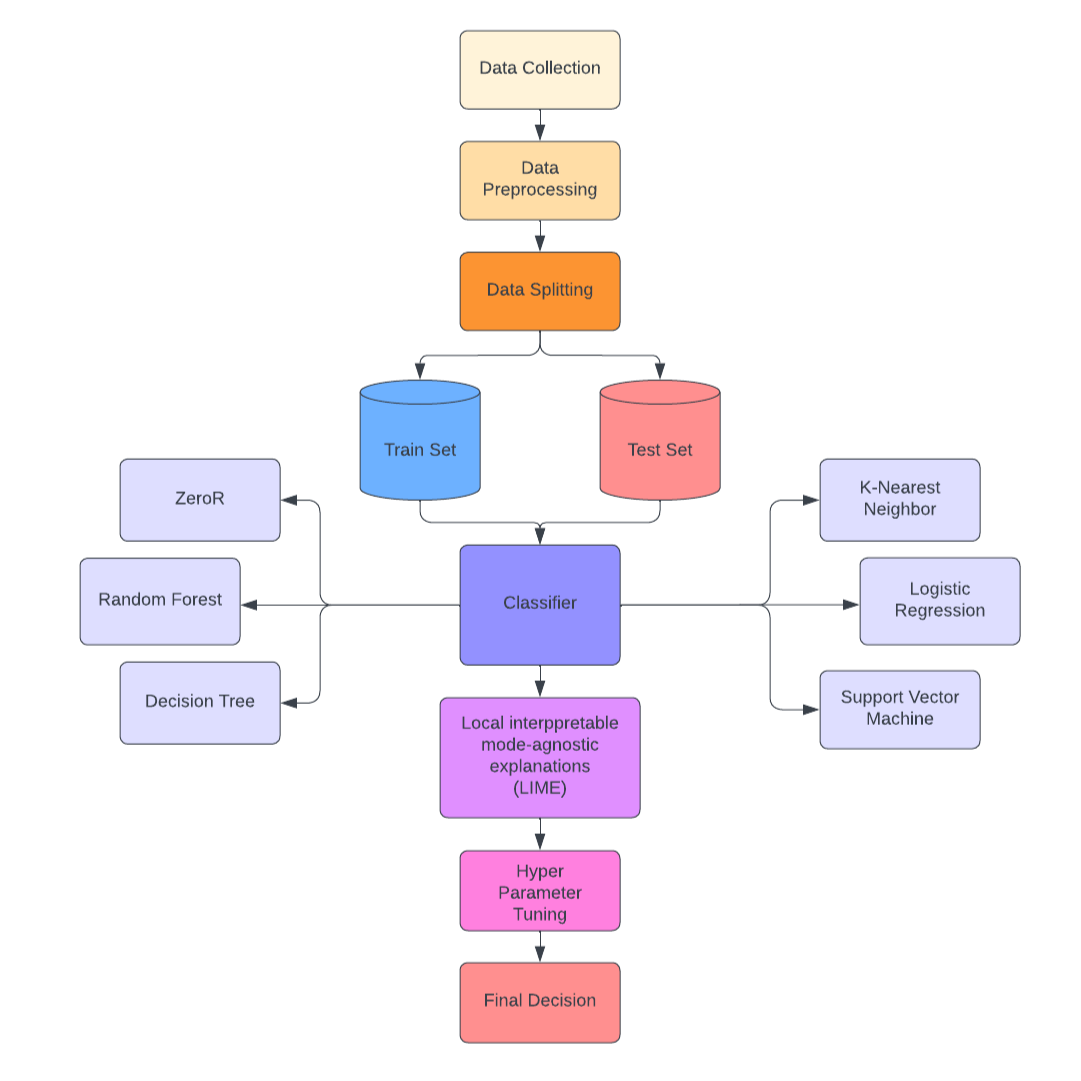
\includegraphics[width=8cm]{fig1.png}
    \caption{Methodology}
    \label{fig:1}
\end{figure}

\textbf{a)} \textbf{Dataset Acquisition and Description:} 
This dataset offers comprehensive information on student achievement in secondary education across two Portuguese schools. It covers various aspects, including grades, demographics, social factors, and school-related features. The dataset is divided into files for the Math and Portuguese language courses to aid analysis. It encompasses a wide range of attributes, such as school details, student demographics (age, sex, address), family background (family size, parents' cohabitation status, parents' education), parents' occupations, school selection reasons, guardianship, travel time, study time, past class failures, educational support, extracurricular activities, nursery attendance, aspirations for higher education, internet access, relationships, free time, socializing habits, alcohol consumption, health status, and school absences.\par
In addition to these attributes, each course has three grade attributes: G1 (first-period score), G2 (second-period score), and G3 (final score). G3 strongly correlates with G2 and G1, representing the final year score, while G1 and G2 correspond to earlier period grades. Although predicting G3 without considering G1 and G2 presents a challenge, it holds practical significance.\par
This dataset provides valuable insights into the factors influencing student achievement in secondary education, particularly within the Portuguese educational system. The files have been merged into a single CSV file for further analysis, with final grades categorized as 'good' (15-20), 'fair' (10-14), and 'poor' (0-9). Table 2 summarizes both datasets, highlighting no class imbalance in the target variable 'final grade.'

\FloatBarrier
\begin{table}[hbt!]
\label{table2}
\centering
\caption{Dataset summary}
\begin{tabular}{|p{1cm}|p{1cm}|p{1cm}|p{1cm}|p{1cm}|p{1cm}| }
\hline
Dataset & Number of Instances & Number of Features& Poor & Fair & Good\\ \hline
Student Performance & 1044 & 32 & 230 & 610 & 204 \\ \hline 
\end{tabular}
\end{table}

\textbf{b)} \textbf{Data prepossessing:} To enhance readability, we improved the column names for better understanding. We implemented feature engineering techniques, including creating the 'final grade' feature, which transformed numerical final scores into categorical variables based on specific ranges. Our careful examination of the dataset ensured no errors or missing values. The data pre-processing phase involved four steps. Firstly, we addressed missing data and then transformed categorical data into numeric using the One-Hot Encoding approach from Scikit-learn. While Decision Trees handle categorical data well, most algorithms perform better with numeric data. To address numeric features with varying ranges, we performed Min-Max Scaling for data normalization, rescaling values from 0 to 1 to enable comparability across features while preserving relationships between data points. After encoding and scaling, we created a new data frame, excluding the 'final score' feature since it had already been converted to 'final grade' to prevent it from influencing predictions in the classification task. Additionally, we converted the categorical values in the 'final grade' column to numerical representation using a mapping dictionary, ensuring compatibility with classification algorithms and simplifying analysis and prediction processes. To gain insights into feature relationships, we analyzed the correlation matrix, revealing strong dependencies between predictions and first/second-period scores and significant correlations with parents' education, study time, and final grades.
 
\begin{figure}[H]
    \centering
    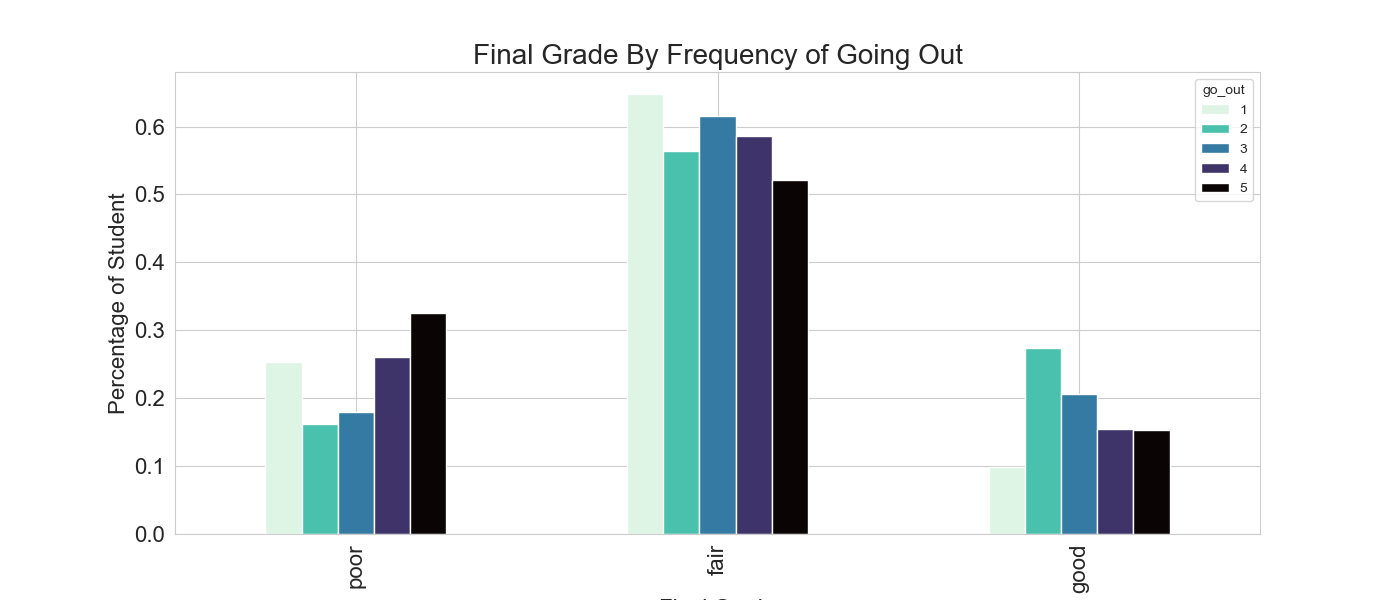
\includegraphics[width=8cm]{fig2.png}
    \caption{Final Grade By Frequency of Going Out}
    \label{fig:2}
\end{figure}

\begin{figure}[H]
    \centering
    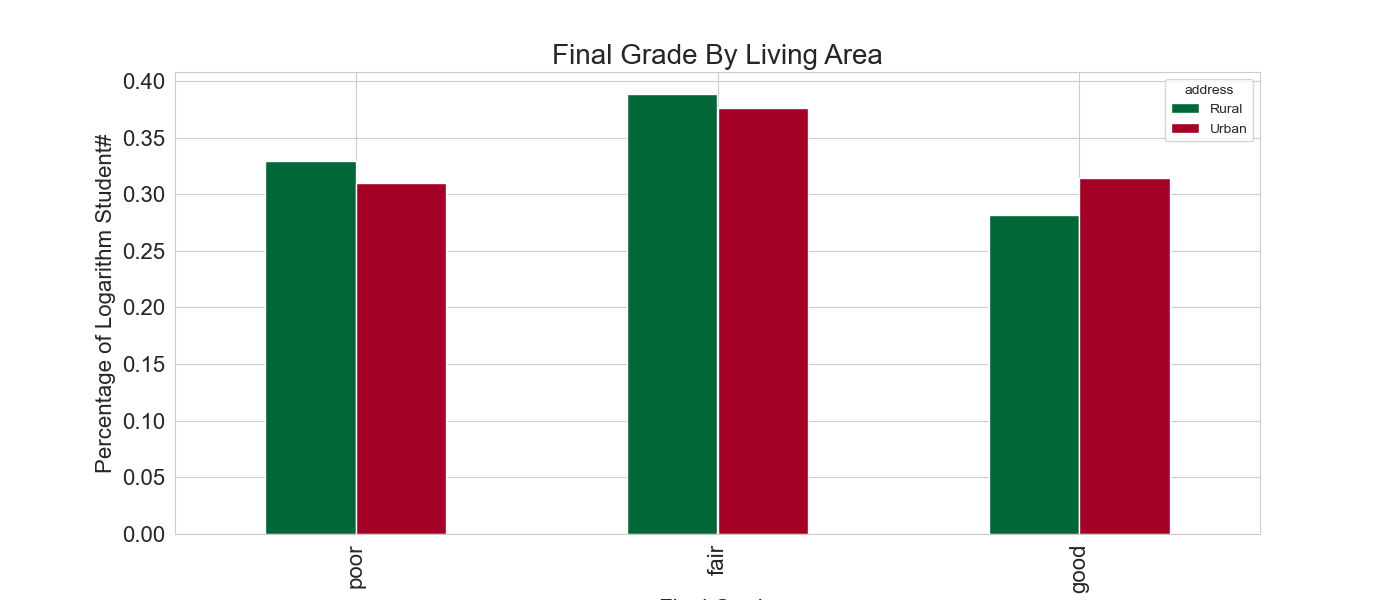
\includegraphics[width=8cm]{fig3.png}
    \caption{Final Grade By Living Area }
    \label{fig:3}
\end{figure}

\begin{figure}[H]
    \centering
    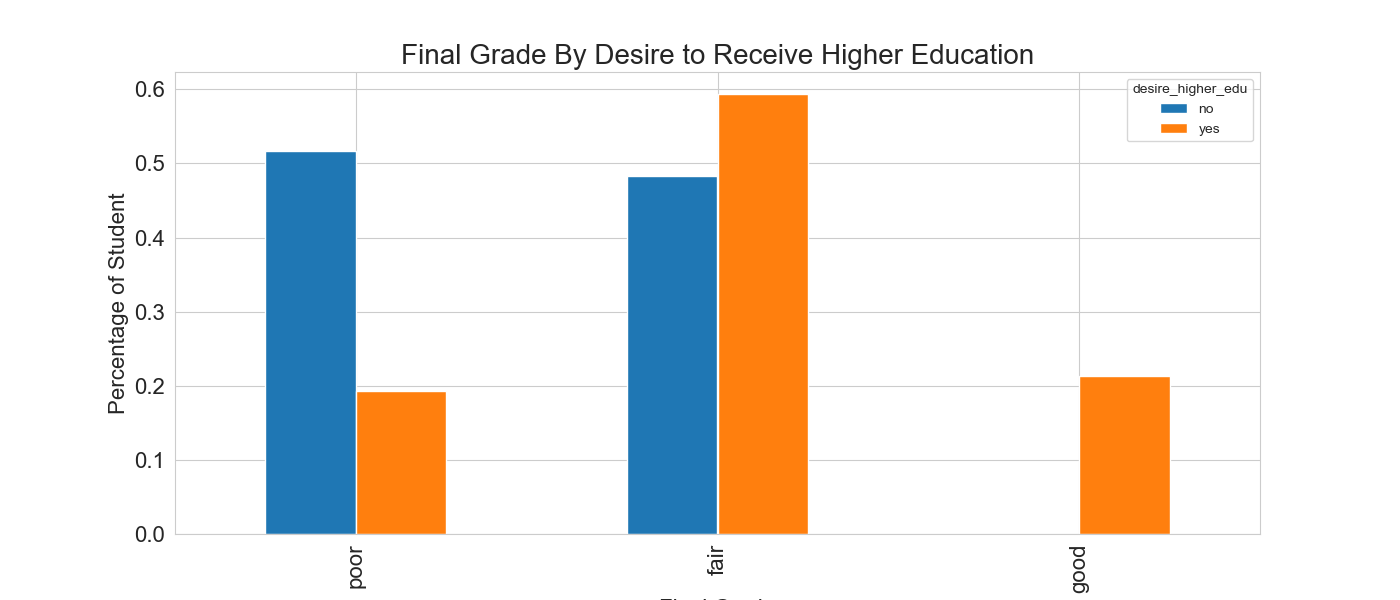
\includegraphics[width=8cm]{fig4.png}
    \caption{Final Grade By Desire to Receive Higher Education}
    \label{fig:4}
\end{figure}


\begin{figure}[H]
    \centering
    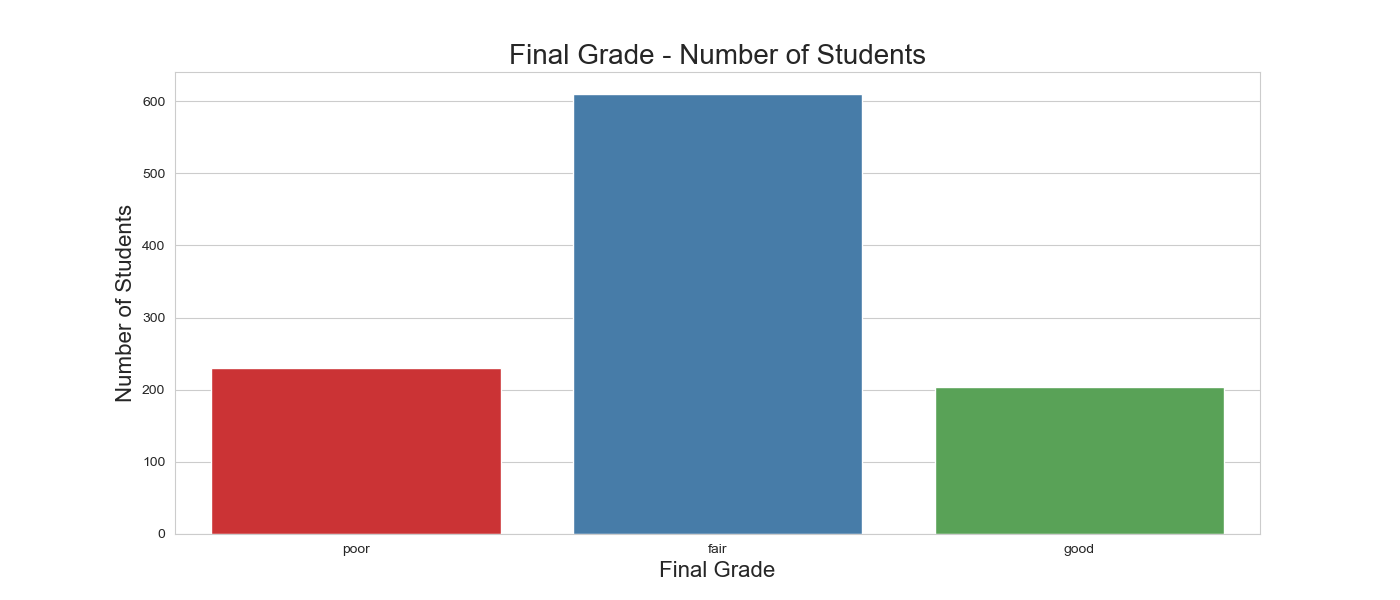
\includegraphics[width=8cm]{fig5.png}
    \caption{Final Grade By Number of Students}
    \label{fig:5}
\end{figure}

\textbf{c)} \textbf{Data Splitting:}
Data splitting is crucial in evaluating classification models, enabling us to assess their performance on new and unseen data. The dataset is divided into two parts: a training set and a testing set. During training, the model learns patterns and relationships within the data, while the testing set remains unseen until evaluation. To ensure fairness and accuracy, we employ stratified sampling, maintaining the distribution of classes in the target variable across both sets. This prevents biases that could arise from imbalanced class distributions. The widely-used train test split function from the scikit-learn library is employed for data splitting, allowing us to specify the desired ratio of 70 percent for training and 30 percent for testing. By incorporating stratified sampling, we achieve an unbiased evaluation of the model's performance and mitigate the risk of overfitting, ensuring the model's ability to generalize well to new and unseen data.\par
\vspace{3mm}
\textbf{d)} \textbf{Classifier:}
Once the data pre-processing and splitting steps are done in the classifier stage, the data is prepared for the machine learning classifiers. In our work, we evaluated several classifiers: ZeroR, Decision tree, Random forest, K-Nearest neighbor, Logistic Regression, and Support Vector Machine. Among these classifiers, Decision trees, K-Nearest neighbors, and Random forests require hyper-parameter tuning for optimal performance. To achieve this, we performed hyper-parameter tuning for each classifier using a three-fold cross-validation on the training set.\par

Brief descriptions of the classifiers are provided as follows. 
\begin{itemize}
\item \textbf{ZeroR}:\par ZeroR is the simplest of the rule-based classifiers, which rely on the target and ignore all predictors. It simply predicts the majority class. It is based on Frequency Table. The ZeroR classifier takes a look at the target attribute and its possible values. It constructs the frequency table and selects its most frequent value. It will ever output the value that is most frequently found for the target attribute in the given dataset. ZeroR, as its name suggests, it does not include any rule that works on the non-target attributes. So more specifically, it predicts the mean (for a numeric type target attribute) or the mode (for a nominal type attribute).
\vspace{3mm}
\item \textbf{Decision Tree:}\par A decision tree is a model that has a tree structure describing the possible states corresponding to events. In machine learning, Decision Tree is a non-parametric supervised learning method that is often applied to solve classification and regression problems. The idea of learning to build a decision tree is to divide the training set into smaller subsets, in which each subset is as "pure" as possible. The purity of a particular set is determined by the number of training elements that have the same class label. In fact, decision trees are built using algorithms Hunts, ID3, C4.5, and J48 is an implementation version of C4.5 in 19 Weka software. This algorithm is based on the Entropy and the information gains concept.\par
\begin{equation} \label{eq1}
E(S) = \sum - p_ilog_2p_jc_j = 1\
\end{equation}


\vspace{3mm}
\item \textbf{Random Forest (RF):}\par The Random Forest boosts the performance of single simple decision trees by bootstrap aggregating algorithm. Particularly, Random Forest uses multiple versions of the training set created by bootstrapping the original training data to train the different decision tree models. In the classification process, for each new instance that needs classification, the final decision is formed by a voting process from all simple decision tree classifiers.
\vspace{3mm}
\item \textbf{K-Nearest Neighbor (KNN):}\par A simple, non-parametric supervised learning algorithm is the K-Nearest Neighbor algorithm, which can be used for both regression and classification. Based on the feature similarity (e.g., distance function), all the available cases are stored, and new cases are classified by it. The output is a class member in the KNN classification. A case is categorized by a predominance vote of its neighbors. The case is allotted to the utmost common class among its K-nearest neighbors. Various heuristic techniques can select the value of K (positive integer) in the KNN method. The case will be assigned to the class of its nearest neighbor if K=1. Different distance functions like Minkowski Distance, Manhattan Distance, and Euclidean Distance are used in the KNN algorithm. In this work, the Minkowski Distance function has been used. The Minkowski Distance for two points U (u1, u2, ...., un) and V (v1, v2, ...., vn) can be represented by the following equation, where q represents the order of the Minkowski Distance.\par
\begin{equation} \label{eq2}
distance(U, V) = (\sum_{i=1}^{n} ((|u_i - v_i|)^q)^\frac{1}{q}\
\end{equation}
\vspace{3mm}
\item \textbf{Logistic Regression:}\par Logistic Regression represents a mathematical modeling technique that describes the relationship between several independent variables, Z1...Zn, and a dependent variable, D. The logistic model uses the logistic function as a mathematical form which has the range between 0 and 1 for any given input. The logistic model can describe a probability of an event which is always a value between 0 and 1. The following formula represents the logistic model.\par 

\begin{equation} \label{eq3}
y=\alpha_0 + \alpha_1 Z_1 + \alpha_2 Z_2 + ... + \alpha_n Z_n\
\end{equation}

Here y is the response variable, and Z1, Z2,…Zn is the predicted variable. By applying the 20 sigmoid functions, we can get the logistic function.\par
\begin{equation} \label{eq4}
l = \frac{1}{1 + e^{-^(\alpha_0 + \alpha_1 Z_1 + \alpha_2 Z_2 + ... + \alpha_n Z_n)}}\
\end{equation}
\vspace{3mm}
\item \textbf{Support Vector Machine (SVM):}\par Support Vector Machine (SVM) tries to separate two classes using an optimal hyperplane. It uses supervised learning. SVM works better if the size of the data is small. It attempts to make the decision boundary to such a degree that the partition between two 18 classes is as broad as could reasonably be expected. To separate two classes, let’s assume we are given a training dataset, D= (x1, C1), (x2, C2), ..., (xn, Cn) where xi denotes the input vector, and Ci refers to the class label of the vector which could be specified as either positive or negative. For specifying any unspecified vector X, the condition is as follows:\par
\begin{equation} \label{eq5}
f(X) = \sum_{i=1}^{N} a_iC_i(x_i^T X) + b\
\end{equation}
Here, the bias is represented by b.
\end{itemize}
\vspace{3mm}
\textbf{e)} \textbf{Hyper-parameter tuning:}\par
Hyperparameters and thus, this process of searching for the ideal model architecture is referred to as hyperparameter tuning. These hyperparameters are used to improve the learning of the model, and their values are set before starting the learning process of the model. Grid search is arguably the most basic hyperparameter tuning method. With this technique, we simply build a model for each possible combination of all of the hyperparameter values provided, evaluating each model and selecting the architecture which produces the best results. Random search differs from grid search in that we longer provide a discrete set of values to explore for each hyperparameter; rather, we provide a statistical distribution for each hyperparameter from which values may be randomly sampled.

\section{Results}
This section elaborates on the classifiers carried out to test and evaluates the proposed model.

\begin{figure}[H]
    \centering
    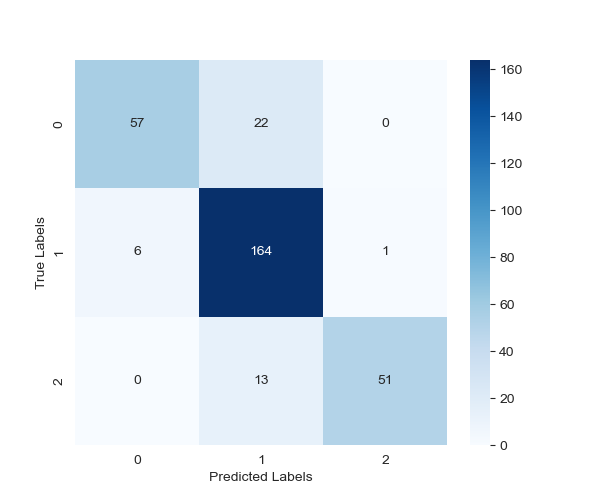
\includegraphics[width=8cm]{fig6.png}
    \caption{ZeroR confusion matrix}
    \label{fig:6}
\end{figure}

\begin{figure}[H]
    \centering
    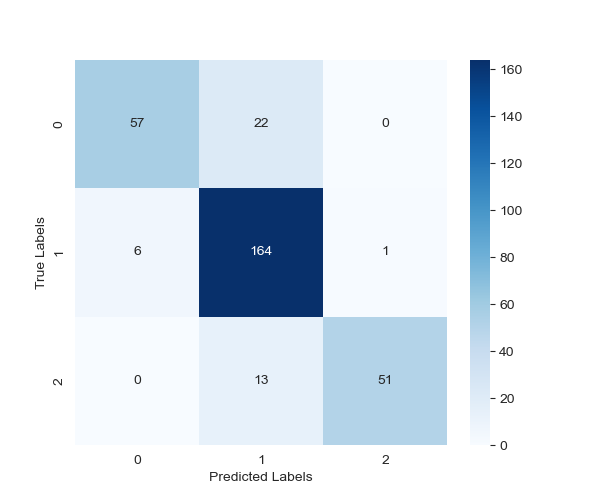
\includegraphics[width=8cm]{fig7.png}
    \caption{Decision Tree confusion matrix}
    \label{fig:7}
\end{figure}

\begin{figure}[H]
    \centering
    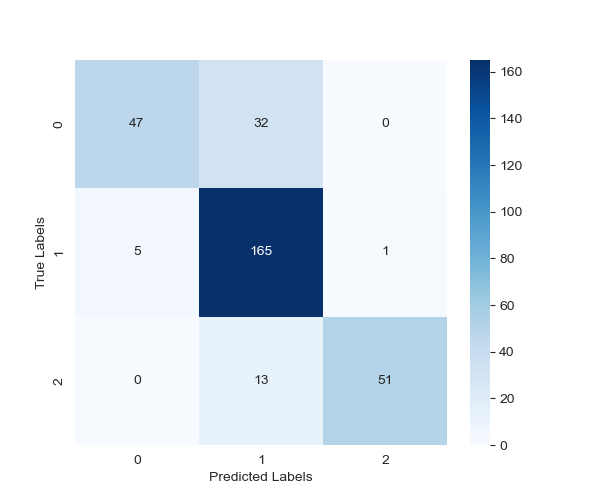
\includegraphics[width=8cm]{fig8.png}
    \caption{Random Forest confusion matrix}
    \label{fig:8}
\end{figure}


\begin{figure}[H]
    \centering
    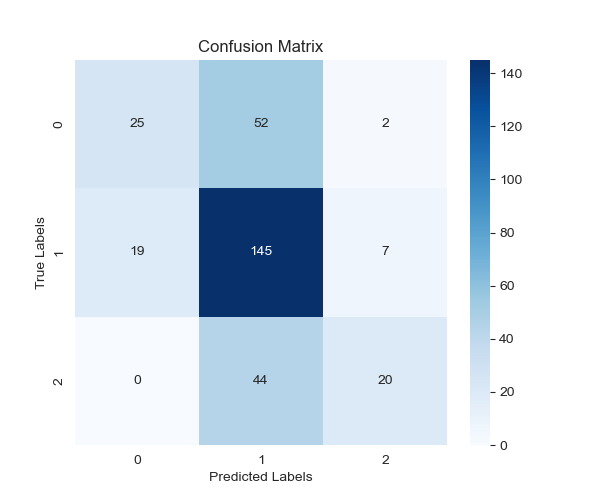
\includegraphics[width=8cm]{fig9.png}
    \caption{K-Nearest Neighbor(KNN) confusion matrix}
    \label{fig:9}
\end{figure}

\begin{figure}[H]
    \centering
    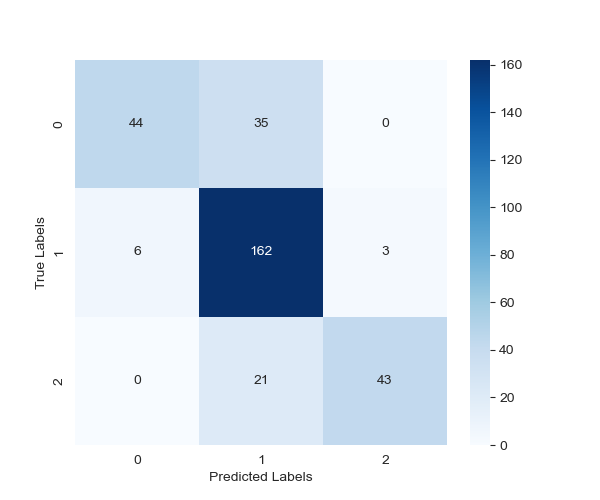
\includegraphics[width=8cm]{fig10.png}
    \caption{Logistic Regression confusion matrix}
    \label{fig:10}
\end{figure}

\begin{figure}[H]
    \centering
    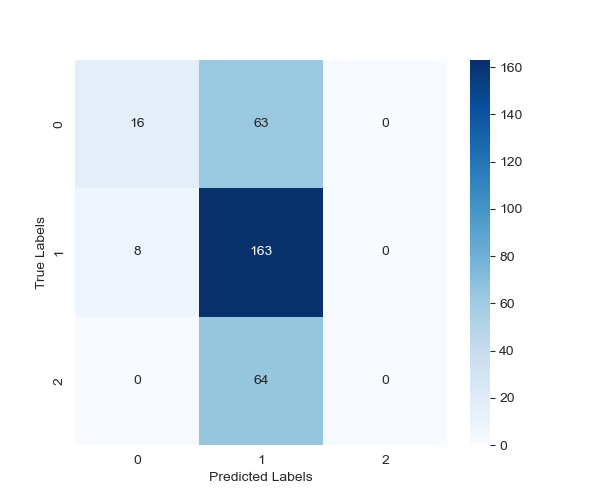
\includegraphics[width=8cm]{fig11.png}
    \caption{Support Vector Machine(SVM) confusion matrix}
    \label{fig:11}
\end{figure}

For testing purposes, 30 percent of the dataset have been used. Figure 6-11 displays the confusion matrix for Student Performance dataset. The confusion matrix was used to define the performance of a classification algorithm as well as visualize and summarize the performance of a classification algorithm. We calculated the accuracy, precision, recall, F1-score scores from this confusion matrices using the following equations:\par
\vspace{3mm}
\textbf{Accuracy =} (TP + TN) / (TP + TN + FP + FN)

\textbf{Precision =} (TP) / (TP + FP)

\textbf{Recall =} (TP) / (TP + FN)

\textbf{F-Measure =} (2 * Precision * Recall) / (Precision + Recall)



TP = True Positive

TN = True Negative

FP = False Positive

FN = False Negative

\FloatBarrier
\begin{table}[hbt!]
\label{table3}
\centering
\caption{Comparison of classification reports evaluated by Student Performance Dataset}
\begin{tabular} {|p{1cm}|p{1cm}|p{1cm}|p{1cm}|p{1cm}|p{1cm}|p{1cm}|}
\hline
Dataset& Classifier Name & Accuracy& Precision&Recall&F1-score &AUC\\\hline
Student Performance & ZeroR & 0.87  &  0.88 &  0.83 & 0.86 & -\\ \hline 
Student Performance& KNN & 0.61  & 0.62 & 0.61 & 0.57
& 0.72\\ \hline
Student Performance & Random Forest & 0.82  & 0.85 &0.83&0.82 &0.94 \\ \hline
Student Performance& Decision Tree & 0.87  & 0.88&0.87& 0.86 &0.94\\ \hline
Student Performance& SVC & 0.57  & 0.47 &0.57&0.6 &-\\ \hline
Student Performance & Logistic Regression & 0.79  & 0.82 &0.79&0.78 &0.91 \\ \hline
\end{tabular}
\end{table}

\begin{figure}[H]
    \centering
    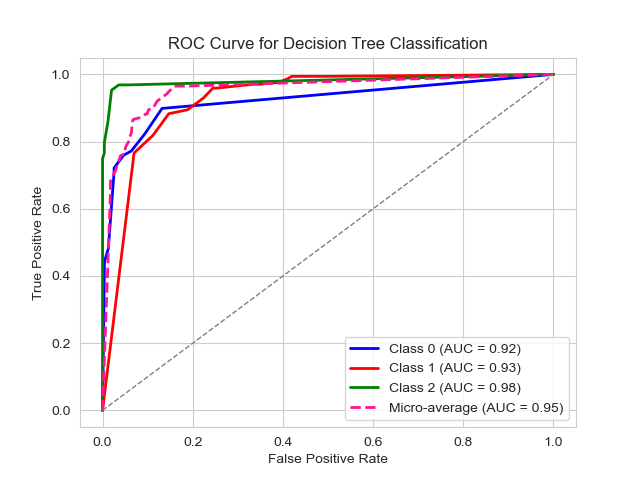
\includegraphics[width=8cm]{fig12.png}
    \caption{ROC curve for Decision Tree Classification}
    \label{fig:12}
\end{figure}

\begin{figure}[H]
    \centering
    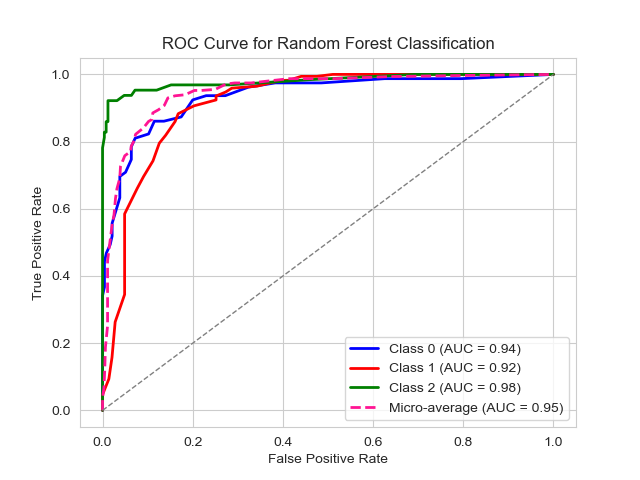
\includegraphics[width=8cm]{fig13.png}
    \caption{ROC curve for Random forest Classification}
    \label{fig:13}
\end{figure}

\begin{figure}[H]
    \centering
    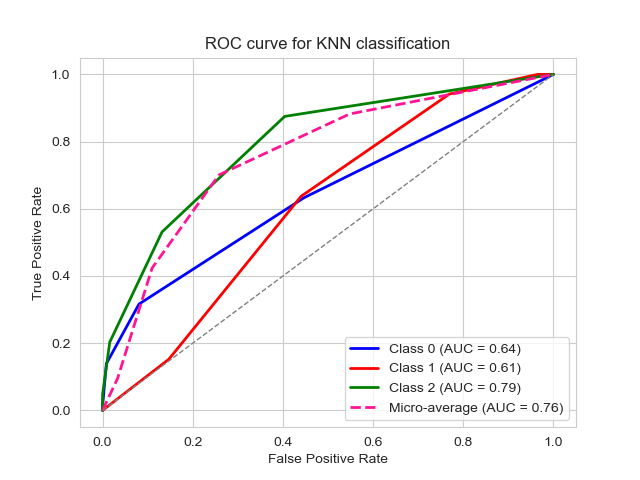
\includegraphics[width=8cm]{fig14.png}
    \caption{ROC curve for KNN Classification}
    \label{fig:14}
\end{figure}

\begin{figure}[H]
    \centering
    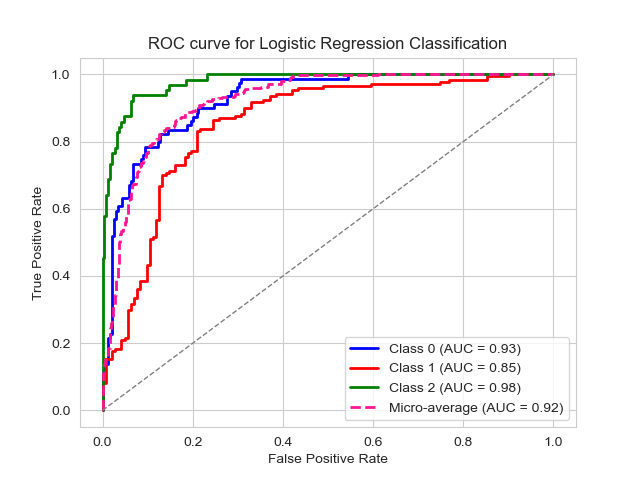
\includegraphics[width=8cm]{fig15.png}
    \caption{ROC curve for Logistic Regression Classification}
    \label{fig:15}
\end{figure}

Figure 12-15 displays the ROC curve comparison of our four classifiers for the Student Performance dataset. A ROC curve (receiver operating characteristic curve) is a graph showing the performance of a classification model at all classification thresholds. This curve plots two parameters: True Positive Rate and False Positive Rate, where True Positive Rate is on the y-axis and False Positive Rate is on the x-axis. The area under the ROC curve is called AUC. A higher AUC (Area under the ROC Curve) indicates a better model for predicting outputs. From the table-3, it is obvious that the Decision tree classifier and Random Forest performed best while testing with the performance dataset, and the highest area under the ROC curve was obtained.

\begin{figure}[H]
    \centering
    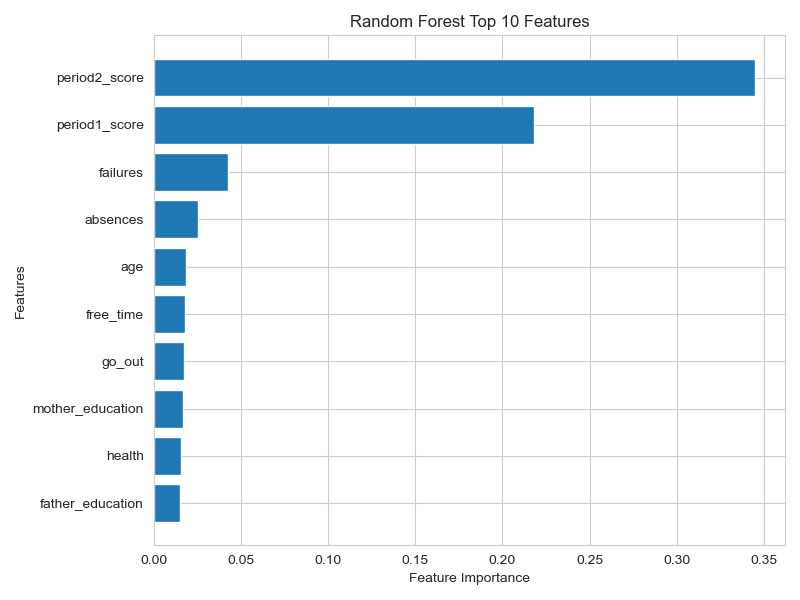
\includegraphics[width=8cm]{fig17.png}
    \caption{Random Forest Top 10 Features}
    \label{fig:17}
\end{figure}

\begin{figure}[H]
    \centering
    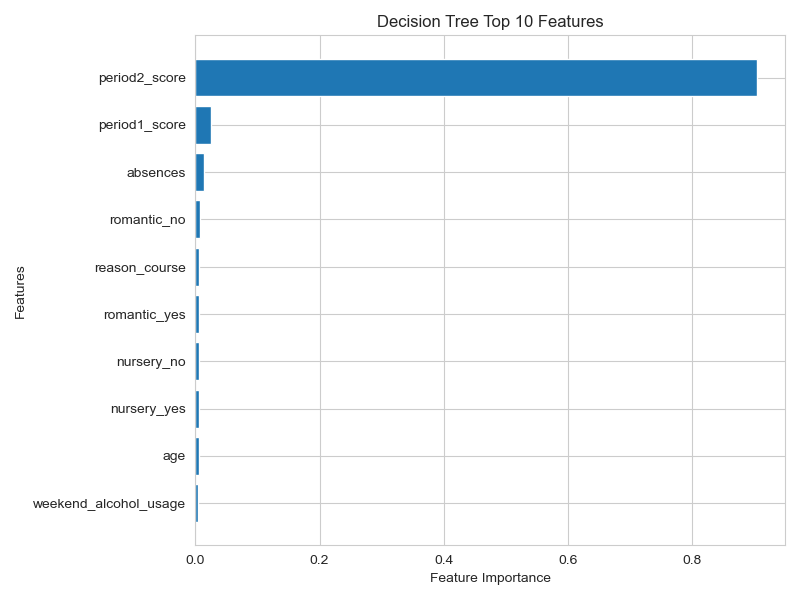
\includegraphics[width=8cm]{fig18.png}
    \caption{Decission Tree Top 10 Features}
    \label{fig:18}
\end{figure}
\section{Discussion}
We have attained the research goals from the empirical results. We identified the variables that influence education success in high school students. Two of the machine learning classifiers predicted the performance with great accuracy.

\section{Conclusion}
This paper presents a data-driven approach to understanding different factors affecting the academic performance of Bangladeshi students. This study has used six classifiers to predict the students’ performance. A comparison between six machine learning algorithms in the realms of academic performance prediction has been made. The algorithms predicted academic performance with varying degrees of accuracy. It was found that the decision tree with hyperparameter tuning performed the best with 87 percent accuracy on the test set. In the future, we plan to collect an enormous dataset from all over Bangladesh. We look forward to exploring the effectiveness of ensemble learning methods on our collected dataset.
\bibliographystyle{ieeetr}
\bibliography{reference}
\vspace{12pt}
\color{red}


\end{document}
